\documentclass[twoside]{book}

% Packages required by doxygen
\usepackage{fixltx2e}
\usepackage{calc}
\usepackage{doxygen}
\usepackage[export]{adjustbox} % also loads graphicx
\usepackage{graphicx}
\usepackage[utf8]{inputenc}
\usepackage{makeidx}
\usepackage{multicol}
\usepackage{multirow}
\PassOptionsToPackage{warn}{textcomp}
\usepackage{textcomp}
\usepackage[nointegrals]{wasysym}
\usepackage[table]{xcolor}

% Font selection
\usepackage[T1]{fontenc}
\usepackage[scaled=.90]{helvet}
\usepackage{courier}
\usepackage{amssymb}
\usepackage{sectsty}
\renewcommand{\familydefault}{\sfdefault}
\allsectionsfont{%
  \fontseries{bc}\selectfont%
  \color{darkgray}%
}
\renewcommand{\DoxyLabelFont}{%
  \fontseries{bc}\selectfont%
  \color{darkgray}%
}
\newcommand{\+}{\discretionary{\mbox{\scriptsize$\hookleftarrow$}}{}{}}

% Page & text layout
\usepackage{geometry}
\geometry{%
  a4paper,%
  top=2.5cm,%
  bottom=2.5cm,%
  left=2.5cm,%
  right=2.5cm%
}
\tolerance=750
\hfuzz=15pt
\hbadness=750
\setlength{\emergencystretch}{15pt}
\setlength{\parindent}{0cm}
\setlength{\parskip}{3ex plus 2ex minus 2ex}
\makeatletter
\renewcommand{\paragraph}{%
  \@startsection{paragraph}{4}{0ex}{-1.0ex}{1.0ex}{%
    \normalfont\normalsize\bfseries\SS@parafont%
  }%
}
\renewcommand{\subparagraph}{%
  \@startsection{subparagraph}{5}{0ex}{-1.0ex}{1.0ex}{%
    \normalfont\normalsize\bfseries\SS@subparafont%
  }%
}
\makeatother

% Headers & footers
\usepackage{fancyhdr}
\pagestyle{fancyplain}
\fancyhead[LE]{\fancyplain{}{\bfseries\thepage}}
\fancyhead[CE]{\fancyplain{}{}}
\fancyhead[RE]{\fancyplain{}{\bfseries\leftmark}}
\fancyhead[LO]{\fancyplain{}{\bfseries\rightmark}}
\fancyhead[CO]{\fancyplain{}{}}
\fancyhead[RO]{\fancyplain{}{\bfseries\thepage}}
\fancyfoot[LE]{\fancyplain{}{}}
\fancyfoot[CE]{\fancyplain{}{}}
\fancyfoot[RE]{\fancyplain{}{\bfseries\scriptsize Generated by Doxygen }}
\fancyfoot[LO]{\fancyplain{}{\bfseries\scriptsize Generated by Doxygen }}
\fancyfoot[CO]{\fancyplain{}{}}
\fancyfoot[RO]{\fancyplain{}{}}
\renewcommand{\footrulewidth}{0.4pt}
\renewcommand{\chaptermark}[1]{%
  \markboth{#1}{}%
}
\renewcommand{\sectionmark}[1]{%
  \markright{\thesection\ #1}%
}

% Indices & bibliography
\usepackage{natbib}
\usepackage[titles]{tocloft}
\setcounter{tocdepth}{3}
\setcounter{secnumdepth}{5}
\makeindex

% Hyperlinks (required, but should be loaded last)
\usepackage{ifpdf}
\ifpdf
  \usepackage[pdftex,pagebackref=true]{hyperref}
\else
  \usepackage[ps2pdf,pagebackref=true]{hyperref}
\fi
\hypersetup{%
  colorlinks=true,%
  linkcolor=blue,%
  citecolor=blue,%
  unicode%
}

% Custom commands
\newcommand{\clearemptydoublepage}{%
  \newpage{\pagestyle{empty}\cleardoublepage}%
}

\usepackage{caption}
\captionsetup{labelsep=space,justification=centering,font={bf},singlelinecheck=off,skip=4pt,position=top}

%===== C O N T E N T S =====

\begin{document}

% Titlepage & ToC
\hypersetup{pageanchor=false,
             bookmarksnumbered=true,
             pdfencoding=unicode
            }
\pagenumbering{alph}
\begin{titlepage}
\vspace*{7cm}
\begin{center}%
{\Large Gaia DB \\[1ex]\large 0.\+9 }\\
\vspace*{1cm}
{\large Generated by Doxygen 1.8.14}\\
\end{center}
\end{titlepage}
\clearemptydoublepage
\pagenumbering{roman}
\tableofcontents
\clearemptydoublepage
\pagenumbering{arabic}
\hypersetup{pageanchor=true}

%--- Begin generated contents ---
\chapter{Class Index}
\section{Class List}
Here are the classes, structs, unions and interfaces with brief descriptions\+:\begin{DoxyCompactList}
\item\contentsline{section}{\mbox{\hyperlink{struct__db__ctx}{\+\_\+db\+\_\+ctx}} \\*A small struct which holds pointers to databases and the directory they are in }{\pageref{struct__db__ctx}}{}
\item\contentsline{section}{\mbox{\hyperlink{struct__star}{\+\_\+star}} \\*Star struct which holds basic data of a star }{\pageref{struct__star}}{}
\end{DoxyCompactList}

\chapter{File Index}
\section{File List}
Here is a list of all documented files with brief descriptions\+:\begin{DoxyCompactList}
\item\contentsline{section}{src/\mbox{\hyperlink{database__common_8c}{database\+\_\+common.\+c}} \\*Helper functions for database interaction }{\pageref{database__common_8c}}{}
\item\contentsline{section}{src/\mbox{\hyperlink{database__common_8h}{database\+\_\+common.\+h}} \\*Helper functions for database interaction }{\pageref{database__common_8h}}{}
\item\contentsline{section}{src/\mbox{\hyperlink{gaia__db_8c}{gaia\+\_\+db.\+c}} \\*Implementation of the Berkeley\+DB wrapper }{\pageref{gaia__db_8c}}{}
\item\contentsline{section}{src/\mbox{\hyperlink{gaia__db_8h}{gaia\+\_\+db.\+h}} \\*Gaia DB wrapper }{\pageref{gaia__db_8h}}{}
\end{DoxyCompactList}

\chapter{Class Documentation}
\hypertarget{struct__db__ctx}{}\section{\+\_\+db\+\_\+ctx Struct Reference}
\label{struct__db__ctx}\index{\+\_\+db\+\_\+ctx@{\+\_\+db\+\_\+ctx}}


A small struct which holds pointers to databases and the directory they are in.  




{\ttfamily \#include $<$gaia\+\_\+db.\+hpp$>$}

\subsection*{Public Attributes}
\begin{DoxyCompactItemize}
\item 
\mbox{\Hypertarget{struct__db__ctx_a0ff642d9584a191613fa5aa0bf6c1517}\label{struct__db__ctx_a0ff642d9584a191613fa5aa0bf6c1517}} 
DB $\ast$ \mbox{\hyperlink{struct__db__ctx_a0ff642d9584a191613fa5aa0bf6c1517}{dbp}}
\begin{DoxyCompactList}\small\item\em Handle to the primary database. \end{DoxyCompactList}\item 
\mbox{\Hypertarget{struct__db__ctx_ac2d1ca553302f173bd7d5f7bcf410b17}\label{struct__db__ctx_ac2d1ca553302f173bd7d5f7bcf410b17}} 
DB $\ast$ \mbox{\hyperlink{struct__db__ctx_ac2d1ca553302f173bd7d5f7bcf410b17}{sdbp}}
\begin{DoxyCompactList}\small\item\em Handle to the secondary database that holds indices for the morton codes. \end{DoxyCompactList}\item 
\mbox{\Hypertarget{struct__db__ctx_a05f5aef209afa76ebbf4178abea01263}\label{struct__db__ctx_a05f5aef209afa76ebbf4178abea01263}} 
char $\ast$ \mbox{\hyperlink{struct__db__ctx_a05f5aef209afa76ebbf4178abea01263}{db\+\_\+dir}}
\begin{DoxyCompactList}\small\item\em Home directory the databases are located in. \end{DoxyCompactList}\end{DoxyCompactItemize}


\subsection{Detailed Description}
A small struct which holds pointers to databases and the directory they are in. 

The documentation for this struct was generated from the following file\+:\begin{DoxyCompactItemize}
\item 
src/\mbox{\hyperlink{gaia__db_8hpp}{gaia\+\_\+db.\+hpp}}\end{DoxyCompactItemize}

\hypertarget{struct__star}{}\section{\+\_\+star Struct Reference}
\label{struct__star}\index{\+\_\+star@{\+\_\+star}}


Star struct which holds basic data of a star.  




{\ttfamily \#include $<$gaia\+\_\+db.\+hpp$>$}

\subsection*{Public Attributes}
\begin{DoxyCompactItemize}
\item 
\mbox{\Hypertarget{struct__star_a6b571bc027dfc8c30bad11bfce07a23c}\label{struct__star_a6b571bc027dfc8c30bad11bfce07a23c}} 
u\+\_\+int64\+\_\+t \mbox{\hyperlink{struct__star_a6b571bc027dfc8c30bad11bfce07a23c}{id}}
\begin{DoxyCompactList}\small\item\em ID extracted from dataset. \end{DoxyCompactList}\item 
\mbox{\Hypertarget{struct__star_aa0894b982143e830a7c2b979de63fe69}\label{struct__star_aa0894b982143e830a7c2b979de63fe69}} 
double \mbox{\hyperlink{struct__star_aa0894b982143e830a7c2b979de63fe69}{x}}
\begin{DoxyCompactList}\small\item\em X position star. \end{DoxyCompactList}\item 
\mbox{\Hypertarget{struct__star_a00d87762a797270a59f86b3e5bd82c0e}\label{struct__star_a00d87762a797270a59f86b3e5bd82c0e}} 
double \mbox{\hyperlink{struct__star_a00d87762a797270a59f86b3e5bd82c0e}{y}}
\begin{DoxyCompactList}\small\item\em Y position star. \end{DoxyCompactList}\item 
\mbox{\Hypertarget{struct__star_a07a680ef4c9c4e39d04d7e96722d5eca}\label{struct__star_a07a680ef4c9c4e39d04d7e96722d5eca}} 
double \mbox{\hyperlink{struct__star_a07a680ef4c9c4e39d04d7e96722d5eca}{z}}
\begin{DoxyCompactList}\small\item\em Z position star. \end{DoxyCompactList}\item 
\mbox{\Hypertarget{struct__star_a1d9d46186ac4cb48396d3f4f4126eb80}\label{struct__star_a1d9d46186ac4cb48396d3f4f4126eb80}} 
u\+\_\+int32\+\_\+t \mbox{\hyperlink{struct__star_a1d9d46186ac4cb48396d3f4f4126eb80}{colour}}
\begin{DoxyCompactList}\small\item\em Colour of the star in hex converted to int. \end{DoxyCompactList}\item 
\mbox{\Hypertarget{struct__star_ada0104a0c6633bf55193b3d6e55e6b3c}\label{struct__star_ada0104a0c6633bf55193b3d6e55e6b3c}} 
u\+\_\+int64\+\_\+t \mbox{\hyperlink{struct__star_ada0104a0c6633bf55193b3d6e55e6b3c}{morton\+\_\+index}}
\begin{DoxyCompactList}\small\item\em Morton-\/code of the star in a 3d-\/grid. \end{DoxyCompactList}\end{DoxyCompactItemize}


\subsection{Detailed Description}
Star struct which holds basic data of a star. 

The documentation for this struct was generated from the following file\+:\begin{DoxyCompactItemize}
\item 
src/\mbox{\hyperlink{gaia__db_8hpp}{gaia\+\_\+db.\+hpp}}\end{DoxyCompactItemize}

\chapter{File Documentation}
\hypertarget{database__common_8c}{}\section{src/database\+\_\+common.c File Reference}
\label{database__common_8c}\index{src/database\+\_\+common.\+c@{src/database\+\_\+common.\+c}}


Helper functions for database interaction.  


{\ttfamily \#include \char`\"{}database\+\_\+common.\+h\char`\"{}}\newline
{\ttfamily \#include $<$stdio.\+h$>$}\newline
{\ttfamily \#include $<$stdlib.\+h$>$}\newline
{\ttfamily \#include $<$string.\+h$>$}\newline
{\ttfamily \#include $<$inttypes.\+h$>$}\newline
Include dependency graph for database\+\_\+common.\+c\+:\nopagebreak
\begin{figure}[H]
\begin{center}
\leavevmode
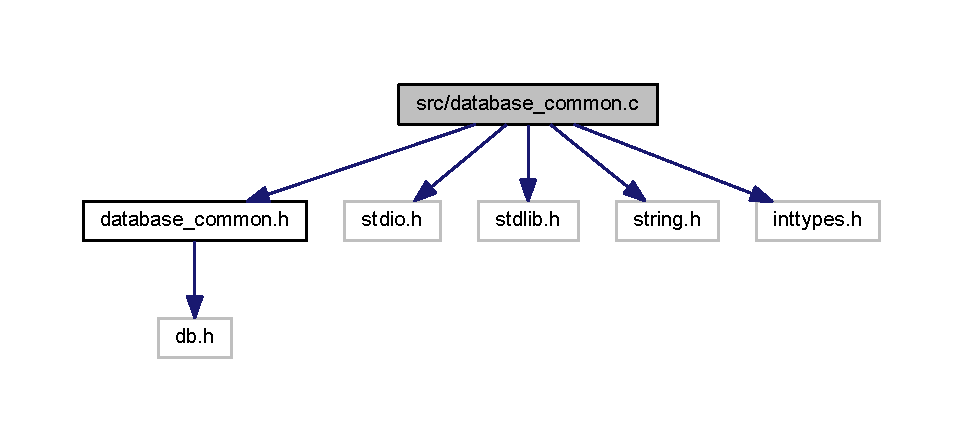
\includegraphics[width=350pt]{database__common_8c__incl}
\end{center}
\end{figure}
\subsection*{Functions}
\begin{DoxyCompactItemize}
\item 
char $\ast$ \mbox{\hyperlink{database__common_8c_af95d1bfd5f0b5c1e72c7f67396675cfe}{make\+\_\+path}} (const char $\ast$str1, const char $\ast$str2)
\begin{DoxyCompactList}\small\item\em Form a path from the string to the directory and the name of the db. This needs to be freed. Done automatically by berkeley if used to create db. \end{DoxyCompactList}\item 
void \mbox{\hyperlink{database__common_8c_a699edc632377de02bf704bd095f2ddca}{log\+\_\+error}} (DB $\ast$dbp, int ret)
\begin{DoxyCompactList}\small\item\em Small helper function for logging errors in the logfile. \end{DoxyCompactList}\item 
int \mbox{\hyperlink{database__common_8c_a81b5fc7e4d1b8bf3aff6d8bbeb4e9795}{db\+\_\+init}} (DB $\ast$$\ast$dbpp, const char $\ast$db\+\_\+directory, const char $\ast$db\+\_\+name, F\+I\+LE $\ast$log\+\_\+file, u\+\_\+int32\+\_\+t db\+\_\+flags, D\+B\+T\+Y\+PE db\+\_\+type)
\begin{DoxyCompactList}\small\item\em Initialize a database. \end{DoxyCompactList}\item 
int \mbox{\hyperlink{database__common_8c_a79a820369077edd8851227043e50df13}{db\+\_\+close}} (DB $\ast$dbp)
\begin{DoxyCompactList}\small\item\em Close the database. \end{DoxyCompactList}\item 
int \mbox{\hyperlink{database__common_8c_a08e70af9ea3c11ceb9141d2ddcba39f0}{db\+\_\+insert}} (DB $\ast$dbp, void $\ast$d\+\_\+key, size\+\_\+t s\+\_\+key, void $\ast$d\+\_\+data, size\+\_\+t s\+\_\+data)
\begin{DoxyCompactList}\small\item\em Insert a value in the database. \end{DoxyCompactList}\item 
void $\ast$ \mbox{\hyperlink{database__common_8c_a6adf5e73a2401b3bf966a3a1aa97a773}{db\+\_\+get}} (DB $\ast$dbp, void $\ast$d\+\_\+key, int s\+\_\+key)
\begin{DoxyCompactList}\small\item\em Get an item from the database. \end{DoxyCompactList}\end{DoxyCompactItemize}


\subsection{Detailed Description}
Helper functions for database interaction. 

\begin{DoxyAuthor}{Author}
Danny Dorstijn 
\end{DoxyAuthor}
\begin{DoxyVersion}{Version}
0.\+9 
\end{DoxyVersion}
\begin{DoxyDate}{Date}
2019-\/01-\/23
\end{DoxyDate}
\begin{DoxyCopyright}{Copyright}
Copyright (c) 2019 
\end{DoxyCopyright}


\subsection{Function Documentation}
\mbox{\Hypertarget{database__common_8c_a79a820369077edd8851227043e50df13}\label{database__common_8c_a79a820369077edd8851227043e50df13}} 
\index{database\+\_\+common.\+c@{database\+\_\+common.\+c}!db\+\_\+close@{db\+\_\+close}}
\index{db\+\_\+close@{db\+\_\+close}!database\+\_\+common.\+c@{database\+\_\+common.\+c}}
\subsubsection{\texorpdfstring{db\+\_\+close()}{db\_close()}}
{\footnotesize\ttfamily int db\+\_\+close (\begin{DoxyParamCaption}\item[{DB $\ast$}]{dbp }\end{DoxyParamCaption})}



Close the database. 


\begin{DoxyParams}{Parameters}
{\em dbp} & -\/ Handle to the db to be closed \\
\hline
\end{DoxyParams}
\begin{DoxyReturn}{Returns}
int -\/ Error code or 0 if all is fine 
\end{DoxyReturn}
\mbox{\Hypertarget{database__common_8c_a6adf5e73a2401b3bf966a3a1aa97a773}\label{database__common_8c_a6adf5e73a2401b3bf966a3a1aa97a773}} 
\index{database\+\_\+common.\+c@{database\+\_\+common.\+c}!db\+\_\+get@{db\+\_\+get}}
\index{db\+\_\+get@{db\+\_\+get}!database\+\_\+common.\+c@{database\+\_\+common.\+c}}
\subsubsection{\texorpdfstring{db\+\_\+get()}{db\_get()}}
{\footnotesize\ttfamily void$\ast$ db\+\_\+get (\begin{DoxyParamCaption}\item[{DB $\ast$}]{dbp,  }\item[{void $\ast$}]{d\+\_\+key,  }\item[{int}]{s\+\_\+key }\end{DoxyParamCaption})}



Get an item from the database. 


\begin{DoxyParams}{Parameters}
{\em dbp} & -\/ Handle to the database \\
\hline
{\em d\+\_\+key} & -\/ Pointer to the key \\
\hline
{\em s\+\_\+key} & -\/ Size of the key \\
\hline
\end{DoxyParams}
\begin{DoxyReturn}{Returns}
void$\ast$ -\/ Data of the record 
\end{DoxyReturn}
\mbox{\Hypertarget{database__common_8c_a81b5fc7e4d1b8bf3aff6d8bbeb4e9795}\label{database__common_8c_a81b5fc7e4d1b8bf3aff6d8bbeb4e9795}} 
\index{database\+\_\+common.\+c@{database\+\_\+common.\+c}!db\+\_\+init@{db\+\_\+init}}
\index{db\+\_\+init@{db\+\_\+init}!database\+\_\+common.\+c@{database\+\_\+common.\+c}}
\subsubsection{\texorpdfstring{db\+\_\+init()}{db\_init()}}
{\footnotesize\ttfamily int db\+\_\+init (\begin{DoxyParamCaption}\item[{DB $\ast$$\ast$}]{dbpp,  }\item[{const char $\ast$}]{db\+\_\+directory,  }\item[{const char $\ast$}]{db\+\_\+name,  }\item[{F\+I\+LE $\ast$}]{log\+\_\+file,  }\item[{u\+\_\+int32\+\_\+t}]{db\+\_\+flags,  }\item[{D\+B\+T\+Y\+PE}]{db\+\_\+type }\end{DoxyParamCaption})}



Initialize a database. 


\begin{DoxyParams}{Parameters}
{\em dbpp} & -\/ A pointer to a handle for the new db \\
\hline
{\em db\+\_\+directory} & -\/ The directory where to place the db \\
\hline
{\em db\+\_\+name} & -\/ Name of the database \\
\hline
{\em log\+\_\+file} & -\/ Log file to print all errors in \\
\hline
{\em db\+\_\+flags} & -\/ Flags for creating a db \\
\hline
{\em db\+\_\+type} & -\/ Type of the db (B\+Tree, Heap, Queue, etc.) \\
\hline
\end{DoxyParams}
\begin{DoxyReturn}{Returns}
int -\/ Error code or 0 if all is fine 
\end{DoxyReturn}
\mbox{\Hypertarget{database__common_8c_a08e70af9ea3c11ceb9141d2ddcba39f0}\label{database__common_8c_a08e70af9ea3c11ceb9141d2ddcba39f0}} 
\index{database\+\_\+common.\+c@{database\+\_\+common.\+c}!db\+\_\+insert@{db\+\_\+insert}}
\index{db\+\_\+insert@{db\+\_\+insert}!database\+\_\+common.\+c@{database\+\_\+common.\+c}}
\subsubsection{\texorpdfstring{db\+\_\+insert()}{db\_insert()}}
{\footnotesize\ttfamily int db\+\_\+insert (\begin{DoxyParamCaption}\item[{DB $\ast$}]{dbp,  }\item[{void $\ast$}]{d\+\_\+key,  }\item[{size\+\_\+t}]{s\+\_\+key,  }\item[{void $\ast$}]{d\+\_\+data,  }\item[{size\+\_\+t}]{s\+\_\+data }\end{DoxyParamCaption})}



Insert a value in the database. 


\begin{DoxyParams}{Parameters}
{\em dbp} & -\/ Handle to the db \\
\hline
{\em d\+\_\+key} & -\/ Pointer to the data of the key \\
\hline
{\em s\+\_\+key} & -\/ Size of the key (using sizeof) \\
\hline
{\em d\+\_\+data} & -\/ Pointer to the data \\
\hline
{\em s\+\_\+data} & -\/ Sizeof the corresponding data (using sizeof) \\
\hline
\end{DoxyParams}
\begin{DoxyReturn}{Returns}
int -\/ Error code or 0 if all is fine 
\end{DoxyReturn}
\mbox{\Hypertarget{database__common_8c_a699edc632377de02bf704bd095f2ddca}\label{database__common_8c_a699edc632377de02bf704bd095f2ddca}} 
\index{database\+\_\+common.\+c@{database\+\_\+common.\+c}!log\+\_\+error@{log\+\_\+error}}
\index{log\+\_\+error@{log\+\_\+error}!database\+\_\+common.\+c@{database\+\_\+common.\+c}}
\subsubsection{\texorpdfstring{log\+\_\+error()}{log\_error()}}
{\footnotesize\ttfamily void log\+\_\+error (\begin{DoxyParamCaption}\item[{DB $\ast$}]{dbp,  }\item[{int}]{ret }\end{DoxyParamCaption})}



Small helper function for logging errors in the logfile. 


\begin{DoxyParams}{Parameters}
{\em dbp} & -\/ Handle to the database \\
\hline
{\em ret} & -\/ The error code to be printed \\
\hline
\end{DoxyParams}
\mbox{\Hypertarget{database__common_8c_af95d1bfd5f0b5c1e72c7f67396675cfe}\label{database__common_8c_af95d1bfd5f0b5c1e72c7f67396675cfe}} 
\index{database\+\_\+common.\+c@{database\+\_\+common.\+c}!make\+\_\+path@{make\+\_\+path}}
\index{make\+\_\+path@{make\+\_\+path}!database\+\_\+common.\+c@{database\+\_\+common.\+c}}
\subsubsection{\texorpdfstring{make\+\_\+path()}{make\_path()}}
{\footnotesize\ttfamily char$\ast$ make\+\_\+path (\begin{DoxyParamCaption}\item[{const char $\ast$}]{str1,  }\item[{const char $\ast$}]{str2 }\end{DoxyParamCaption})}



Form a path from the string to the directory and the name of the db. This needs to be freed. Done automatically by berkeley if used to create db. 


\begin{DoxyParams}{Parameters}
{\em str1} & -\/ First string \\
\hline
{\em str2} & -\/ Second string \\
\hline
\end{DoxyParams}
\begin{DoxyReturn}{Returns}
char$\ast$ -\/ Both strings combined 
\end{DoxyReturn}

\hypertarget{database__common_8h}{}\section{src/database\+\_\+common.h File Reference}
\label{database__common_8h}\index{src/database\+\_\+common.\+h@{src/database\+\_\+common.\+h}}


Helper functions for database interaction.  


{\ttfamily \#include \char`\"{}db.\+h\char`\"{}}\newline
Include dependency graph for database\+\_\+common.\+h\+:\nopagebreak
\begin{figure}[H]
\begin{center}
\leavevmode
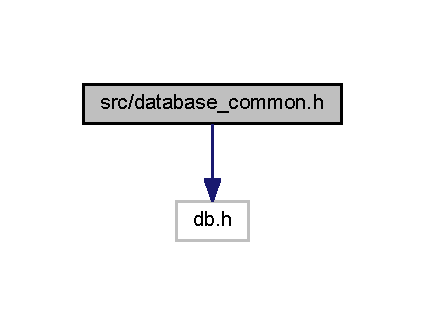
\includegraphics[width=204pt]{database__common_8h__incl}
\end{center}
\end{figure}
This graph shows which files directly or indirectly include this file\+:\nopagebreak
\begin{figure}[H]
\begin{center}
\leavevmode
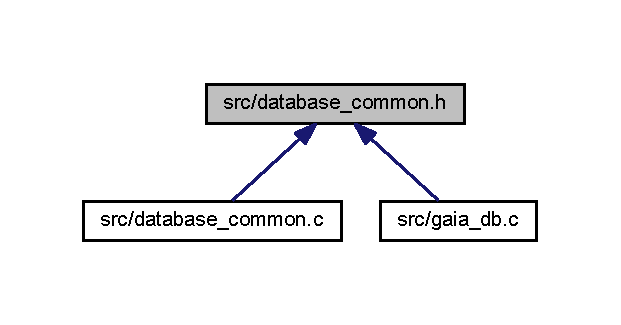
\includegraphics[width=298pt]{database__common_8h__dep__incl}
\end{center}
\end{figure}
\subsection*{Functions}
\begin{DoxyCompactItemize}
\item 
void \mbox{\hyperlink{database__common_8h_a699edc632377de02bf704bd095f2ddca}{log\+\_\+error}} (DB $\ast$dbp, int ret)
\begin{DoxyCompactList}\small\item\em Small helper function for logging errors in the logfile. \end{DoxyCompactList}\item 
int \mbox{\hyperlink{database__common_8h_a81b5fc7e4d1b8bf3aff6d8bbeb4e9795}{db\+\_\+init}} (DB $\ast$$\ast$dbpp, const char $\ast$db\+\_\+directory, const char $\ast$db\+\_\+name, F\+I\+LE $\ast$log\+\_\+file, u\+\_\+int32\+\_\+t db\+\_\+flags, D\+B\+T\+Y\+PE db\+\_\+type)
\begin{DoxyCompactList}\small\item\em Initialize a database. \end{DoxyCompactList}\item 
int \mbox{\hyperlink{database__common_8h_a79a820369077edd8851227043e50df13}{db\+\_\+close}} (DB $\ast$dbp)
\begin{DoxyCompactList}\small\item\em Close the database. \end{DoxyCompactList}\item 
int \mbox{\hyperlink{database__common_8h_a08e70af9ea3c11ceb9141d2ddcba39f0}{db\+\_\+insert}} (DB $\ast$dbp, void $\ast$d\+\_\+key, size\+\_\+t s\+\_\+key, void $\ast$d\+\_\+data, size\+\_\+t s\+\_\+data)
\begin{DoxyCompactList}\small\item\em Insert a value in the database. \end{DoxyCompactList}\item 
void $\ast$ \mbox{\hyperlink{database__common_8h_a6adf5e73a2401b3bf966a3a1aa97a773}{db\+\_\+get}} (DB $\ast$dbp, void $\ast$d\+\_\+key, int s\+\_\+key)
\begin{DoxyCompactList}\small\item\em Get an item from the database. \end{DoxyCompactList}\end{DoxyCompactItemize}


\subsection{Detailed Description}
Helper functions for database interaction. 

\begin{DoxyAuthor}{Author}
Danny Dorstijn 
\end{DoxyAuthor}
\begin{DoxyVersion}{Version}
0.\+9 
\end{DoxyVersion}
\begin{DoxyDate}{Date}
2019-\/01-\/23
\end{DoxyDate}
\begin{DoxyCopyright}{Copyright}
Copyright (c) 2019 
\end{DoxyCopyright}


\subsection{Function Documentation}
\mbox{\Hypertarget{database__common_8h_a79a820369077edd8851227043e50df13}\label{database__common_8h_a79a820369077edd8851227043e50df13}} 
\index{database\+\_\+common.\+h@{database\+\_\+common.\+h}!db\+\_\+close@{db\+\_\+close}}
\index{db\+\_\+close@{db\+\_\+close}!database\+\_\+common.\+h@{database\+\_\+common.\+h}}
\subsubsection{\texorpdfstring{db\+\_\+close()}{db\_close()}}
{\footnotesize\ttfamily int db\+\_\+close (\begin{DoxyParamCaption}\item[{DB $\ast$}]{dbp }\end{DoxyParamCaption})}



Close the database. 


\begin{DoxyParams}{Parameters}
{\em dbp} & -\/ Handle to the db to be closed \\
\hline
\end{DoxyParams}
\begin{DoxyReturn}{Returns}
int -\/ Error code or 0 if all is fine 
\end{DoxyReturn}
\mbox{\Hypertarget{database__common_8h_a6adf5e73a2401b3bf966a3a1aa97a773}\label{database__common_8h_a6adf5e73a2401b3bf966a3a1aa97a773}} 
\index{database\+\_\+common.\+h@{database\+\_\+common.\+h}!db\+\_\+get@{db\+\_\+get}}
\index{db\+\_\+get@{db\+\_\+get}!database\+\_\+common.\+h@{database\+\_\+common.\+h}}
\subsubsection{\texorpdfstring{db\+\_\+get()}{db\_get()}}
{\footnotesize\ttfamily void$\ast$ db\+\_\+get (\begin{DoxyParamCaption}\item[{DB $\ast$}]{dbp,  }\item[{void $\ast$}]{d\+\_\+key,  }\item[{int}]{s\+\_\+key }\end{DoxyParamCaption})}



Get an item from the database. 


\begin{DoxyParams}{Parameters}
{\em dbp} & -\/ Handle to the database \\
\hline
{\em d\+\_\+key} & -\/ Pointer to the key \\
\hline
{\em s\+\_\+key} & -\/ Size of the key \\
\hline
\end{DoxyParams}
\begin{DoxyReturn}{Returns}
void$\ast$ -\/ Data of the record 
\end{DoxyReturn}
\mbox{\Hypertarget{database__common_8h_a81b5fc7e4d1b8bf3aff6d8bbeb4e9795}\label{database__common_8h_a81b5fc7e4d1b8bf3aff6d8bbeb4e9795}} 
\index{database\+\_\+common.\+h@{database\+\_\+common.\+h}!db\+\_\+init@{db\+\_\+init}}
\index{db\+\_\+init@{db\+\_\+init}!database\+\_\+common.\+h@{database\+\_\+common.\+h}}
\subsubsection{\texorpdfstring{db\+\_\+init()}{db\_init()}}
{\footnotesize\ttfamily int db\+\_\+init (\begin{DoxyParamCaption}\item[{DB $\ast$$\ast$}]{dbpp,  }\item[{const char $\ast$}]{db\+\_\+directory,  }\item[{const char $\ast$}]{db\+\_\+name,  }\item[{F\+I\+LE $\ast$}]{log\+\_\+file,  }\item[{u\+\_\+int32\+\_\+t}]{db\+\_\+flags,  }\item[{D\+B\+T\+Y\+PE}]{db\+\_\+type }\end{DoxyParamCaption})}



Initialize a database. 


\begin{DoxyParams}{Parameters}
{\em dbpp} & -\/ A pointer to a handle for the new db \\
\hline
{\em db\+\_\+directory} & -\/ The directory where to place the db \\
\hline
{\em db\+\_\+name} & -\/ Name of the database \\
\hline
{\em log\+\_\+file} & -\/ Log file to print all errors in \\
\hline
{\em db\+\_\+flags} & -\/ Flags for creating a db \\
\hline
{\em db\+\_\+type} & -\/ Type of the db (B\+Tree, Heap, Queue, etc.) \\
\hline
\end{DoxyParams}
\begin{DoxyReturn}{Returns}
int -\/ Error code or 0 if all is fine 
\end{DoxyReturn}
\mbox{\Hypertarget{database__common_8h_a08e70af9ea3c11ceb9141d2ddcba39f0}\label{database__common_8h_a08e70af9ea3c11ceb9141d2ddcba39f0}} 
\index{database\+\_\+common.\+h@{database\+\_\+common.\+h}!db\+\_\+insert@{db\+\_\+insert}}
\index{db\+\_\+insert@{db\+\_\+insert}!database\+\_\+common.\+h@{database\+\_\+common.\+h}}
\subsubsection{\texorpdfstring{db\+\_\+insert()}{db\_insert()}}
{\footnotesize\ttfamily int db\+\_\+insert (\begin{DoxyParamCaption}\item[{DB $\ast$}]{dbp,  }\item[{void $\ast$}]{d\+\_\+key,  }\item[{size\+\_\+t}]{s\+\_\+key,  }\item[{void $\ast$}]{d\+\_\+data,  }\item[{size\+\_\+t}]{s\+\_\+data }\end{DoxyParamCaption})}



Insert a value in the database. 


\begin{DoxyParams}{Parameters}
{\em dbp} & -\/ Handle to the db \\
\hline
{\em d\+\_\+key} & -\/ Pointer to the data of the key \\
\hline
{\em s\+\_\+key} & -\/ Size of the key (using sizeof) \\
\hline
{\em d\+\_\+data} & -\/ Pointer to the data \\
\hline
{\em s\+\_\+data} & -\/ Sizeof the corresponding data (using sizeof) \\
\hline
\end{DoxyParams}
\begin{DoxyReturn}{Returns}
int -\/ Error code or 0 if all is fine 
\end{DoxyReturn}
\mbox{\Hypertarget{database__common_8h_a699edc632377de02bf704bd095f2ddca}\label{database__common_8h_a699edc632377de02bf704bd095f2ddca}} 
\index{database\+\_\+common.\+h@{database\+\_\+common.\+h}!log\+\_\+error@{log\+\_\+error}}
\index{log\+\_\+error@{log\+\_\+error}!database\+\_\+common.\+h@{database\+\_\+common.\+h}}
\subsubsection{\texorpdfstring{log\+\_\+error()}{log\_error()}}
{\footnotesize\ttfamily void log\+\_\+error (\begin{DoxyParamCaption}\item[{DB $\ast$}]{dbp,  }\item[{int}]{ret }\end{DoxyParamCaption})}



Small helper function for logging errors in the logfile. 


\begin{DoxyParams}{Parameters}
{\em dbp} & -\/ Handle to the database \\
\hline
{\em ret} & -\/ The error code to be printed \\
\hline
\end{DoxyParams}

\hypertarget{gaia__db_8c}{}\section{src/gaia\+\_\+db.c File Reference}
\label{gaia__db_8c}\index{src/gaia\+\_\+db.\+c@{src/gaia\+\_\+db.\+c}}


Implementation of the Berkeley\+DB wrapper.  


{\ttfamily \#include \char`\"{}gaia\+\_\+db.\+h\char`\"{}}\newline
{\ttfamily \#include \char`\"{}database\+\_\+common.\+h\char`\"{}}\newline
{\ttfamily \#include $<$stdio.\+h$>$}\newline
{\ttfamily \#include $<$stdlib.\+h$>$}\newline
{\ttfamily \#include $<$string.\+h$>$}\newline
Include dependency graph for gaia\+\_\+db.\+c\+:\nopagebreak
\begin{figure}[H]
\begin{center}
\leavevmode
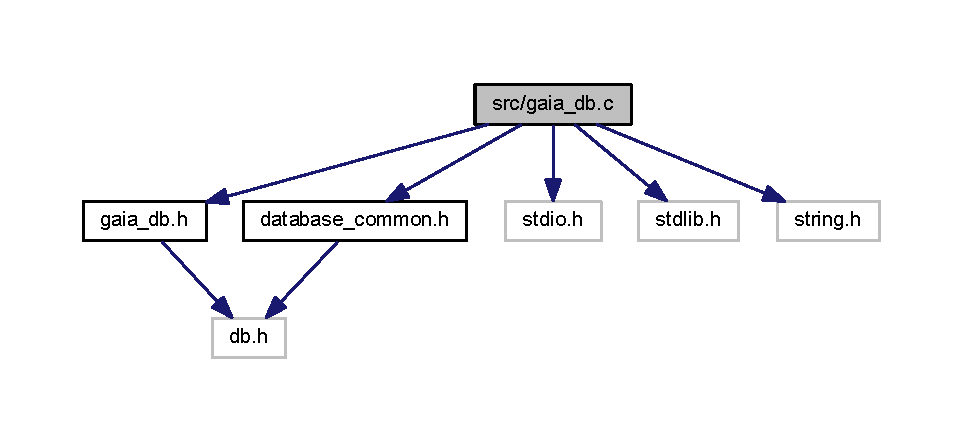
\includegraphics[width=350pt]{gaia__db_8c__incl}
\end{center}
\end{figure}
\subsection*{Functions}
\begin{DoxyCompactItemize}
\item 
int \mbox{\hyperlink{gaia__db_8c_a44e25f43b690896c5c4fa81fbc45d945}{get\+\_\+id\+\_\+callback}} (DB $\ast$dbp, const D\+BT $\ast$pkey, const D\+BT $\ast$pdata, D\+BT $\ast$skey)
\begin{DoxyCompactList}\small\item\em Callback used by the db for creating indices for the morton codes. \end{DoxyCompactList}\item 
\mbox{\hyperlink{gaia__db_8h_a35d505fe9a8343f69d3079cabcf0d402}{D\+B\+\_\+\+C\+TX}} $\ast$ \mbox{\hyperlink{gaia__db_8c_a1fc05df2dfbdc4b7485ee4f7dec123bd}{gaia\+\_\+setup\+\_\+database}} (const char $\ast$directory)
\begin{DoxyCompactList}\small\item\em Setup the databases for G\+A\+IA. \end{DoxyCompactList}\item 
int \mbox{\hyperlink{gaia__db_8c_a1f3af2e6142cee790fe1d91c47213c84}{gaia\+\_\+close\+\_\+database}} (\mbox{\hyperlink{gaia__db_8h_a35d505fe9a8343f69d3079cabcf0d402}{D\+B\+\_\+\+C\+TX}} $\ast$ctx)
\begin{DoxyCompactList}\small\item\em Close the databases. Writes the db\textquotesingle{}s to a file. \end{DoxyCompactList}\item 
int \mbox{\hyperlink{gaia__db_8c_a79dd66ca1c5cbda2845a81ed31abb0aa}{gaia\+\_\+new\+\_\+star}} (DB $\ast$dbp, u\+\_\+int64\+\_\+t id, double x, double y, double z, u\+\_\+int32\+\_\+t colour, float brightness, u\+\_\+int64\+\_\+t morton\+\_\+index)
\item 
\mbox{\hyperlink{gaia__db_8h_af49b70ce88035047e479faabf6e1593f}{S\+Star}} $\ast$ \mbox{\hyperlink{gaia__db_8c_ac0b6ef3a6718a258a142aeb0382fae62}{gaia\+\_\+get\+\_\+star}} (DB $\ast$dbp, u\+\_\+int64\+\_\+t id)
\begin{DoxyCompactList}\small\item\em Get a star from the db based on the ID of the star. \end{DoxyCompactList}\item 
\mbox{\hyperlink{gaia__db_8h_af49b70ce88035047e479faabf6e1593f}{S\+Star}} $\ast$ \mbox{\hyperlink{gaia__db_8c_acf5aafb5995d38f3f3cf7b87702f94a5}{gaia\+\_\+get\+\_\+star\+\_\+by\+\_\+morton}} (DB $\ast$sdbp, u\+\_\+int64\+\_\+t index)
\begin{DoxyCompactList}\small\item\em Get the star based on it\textquotesingle{}s morton code. \end{DoxyCompactList}\item 
D\+BC $\ast$ \mbox{\hyperlink{gaia__db_8c_a7ef90987999253e1c121768ce07e931a}{gaia\+\_\+open\+\_\+cursor}} (DB $\ast$dbp)
\begin{DoxyCompactList}\small\item\em Get a new cursor to iterate over the database. \end{DoxyCompactList}\item 
int \mbox{\hyperlink{gaia__db_8c_ab0dfcb094f0cc2ff4897882597acd265}{gaia\+\_\+close\+\_\+cursor}} (D\+BC $\ast$dbcp)
\begin{DoxyCompactList}\small\item\em Close the cursor after you are done using it. \end{DoxyCompactList}\item 
\mbox{\hyperlink{gaia__db_8h_af49b70ce88035047e479faabf6e1593f}{S\+Star}} $\ast$ \mbox{\hyperlink{gaia__db_8c_a0b340679921c0d83093f53c1b2f0e7c2}{gaia\+\_\+cursor\+\_\+get\+\_\+star}} (D\+BC $\ast$dbcp)
\begin{DoxyCompactList}\small\item\em Get the star the cursor is pointing to. \end{DoxyCompactList}\item 
char \mbox{\hyperlink{gaia__db_8c_a9c5f9643c4403e440334a3f09046626e}{gaia\+\_\+cursor\+\_\+has\+\_\+next}} (D\+BC $\ast$dbcp)
\begin{DoxyCompactList}\small\item\em Check if the cursor is on the last record and jump to that record. \end{DoxyCompactList}\item 
int \mbox{\hyperlink{gaia__db_8c_a480e020be2a5074fb50700acfc53f9f4}{gaia\+\_\+cursor\+\_\+goto\+\_\+star}} (D\+BC $\ast$dbcp, u\+\_\+int64\+\_\+t id)
\begin{DoxyCompactList}\small\item\em Set the cursor to a star with the id given. \end{DoxyCompactList}\item 
int \mbox{\hyperlink{gaia__db_8c_aa607ca1be0f3756cd58d93e7681607ee}{gaia\+\_\+delete\+\_\+star}} (DB $\ast$dbp, u\+\_\+int64\+\_\+t id)
\begin{DoxyCompactList}\small\item\em Search and remove a star from the db. \end{DoxyCompactList}\item 
int \mbox{\hyperlink{gaia__db_8c_a39ba50c931a426c82c882ab6660176f5}{gaia\+\_\+update\+\_\+star\+\_\+morton}} (DB $\ast$dbp, u\+\_\+int64\+\_\+t id, u\+\_\+int64\+\_\+t morton\+\_\+index)
\begin{DoxyCompactList}\small\item\em Update the morton code of the star. \end{DoxyCompactList}\end{DoxyCompactItemize}


\subsection{Detailed Description}
Implementation of the Berkeley\+DB wrapper. 

\begin{DoxyAuthor}{Author}
Danny Dorstijn 
\end{DoxyAuthor}
\begin{DoxyVersion}{Version}
0.\+8 
\end{DoxyVersion}
\begin{DoxyDate}{Date}
2019-\/01-\/23
\end{DoxyDate}
\begin{DoxyCopyright}{Copyright}
Copyright (c) 2019 
\end{DoxyCopyright}


\subsection{Function Documentation}
\mbox{\Hypertarget{gaia__db_8c_ab0dfcb094f0cc2ff4897882597acd265}\label{gaia__db_8c_ab0dfcb094f0cc2ff4897882597acd265}} 
\index{gaia\+\_\+db.\+c@{gaia\+\_\+db.\+c}!gaia\+\_\+close\+\_\+cursor@{gaia\+\_\+close\+\_\+cursor}}
\index{gaia\+\_\+close\+\_\+cursor@{gaia\+\_\+close\+\_\+cursor}!gaia\+\_\+db.\+c@{gaia\+\_\+db.\+c}}
\subsubsection{\texorpdfstring{gaia\+\_\+close\+\_\+cursor()}{gaia\_close\_cursor()}}
{\footnotesize\ttfamily int gaia\+\_\+close\+\_\+cursor (\begin{DoxyParamCaption}\item[{D\+BC $\ast$}]{dbcp }\end{DoxyParamCaption})}



Close the cursor after you are done using it. 


\begin{DoxyParams}{Parameters}
{\em dbcp} & -\/ Handle to the database \\
\hline
\end{DoxyParams}
\begin{DoxyReturn}{Returns}
int -\/ Error code or 0 if all is fine 
\end{DoxyReturn}
\mbox{\Hypertarget{gaia__db_8c_a1f3af2e6142cee790fe1d91c47213c84}\label{gaia__db_8c_a1f3af2e6142cee790fe1d91c47213c84}} 
\index{gaia\+\_\+db.\+c@{gaia\+\_\+db.\+c}!gaia\+\_\+close\+\_\+database@{gaia\+\_\+close\+\_\+database}}
\index{gaia\+\_\+close\+\_\+database@{gaia\+\_\+close\+\_\+database}!gaia\+\_\+db.\+c@{gaia\+\_\+db.\+c}}
\subsubsection{\texorpdfstring{gaia\+\_\+close\+\_\+database()}{gaia\_close\_database()}}
{\footnotesize\ttfamily int gaia\+\_\+close\+\_\+database (\begin{DoxyParamCaption}\item[{\mbox{\hyperlink{gaia__db_8h_a35d505fe9a8343f69d3079cabcf0d402}{D\+B\+\_\+\+C\+TX}} $\ast$}]{ctx }\end{DoxyParamCaption})}



Close the databases. Writes the db\textquotesingle{}s to a file. 


\begin{DoxyParams}{Parameters}
{\em ctx} & -\/ The context with both the database handles \\
\hline
\end{DoxyParams}
\begin{DoxyReturn}{Returns}
int -\/ Returns err code or 0 if all was fine 
\end{DoxyReturn}
\mbox{\Hypertarget{gaia__db_8c_a0b340679921c0d83093f53c1b2f0e7c2}\label{gaia__db_8c_a0b340679921c0d83093f53c1b2f0e7c2}} 
\index{gaia\+\_\+db.\+c@{gaia\+\_\+db.\+c}!gaia\+\_\+cursor\+\_\+get\+\_\+star@{gaia\+\_\+cursor\+\_\+get\+\_\+star}}
\index{gaia\+\_\+cursor\+\_\+get\+\_\+star@{gaia\+\_\+cursor\+\_\+get\+\_\+star}!gaia\+\_\+db.\+c@{gaia\+\_\+db.\+c}}
\subsubsection{\texorpdfstring{gaia\+\_\+cursor\+\_\+get\+\_\+star()}{gaia\_cursor\_get\_star()}}
{\footnotesize\ttfamily \mbox{\hyperlink{gaia__db_8h_af49b70ce88035047e479faabf6e1593f}{S\+Star}}$\ast$ gaia\+\_\+cursor\+\_\+get\+\_\+star (\begin{DoxyParamCaption}\item[{D\+BC $\ast$}]{dbcp }\end{DoxyParamCaption})}



Get the star the cursor is pointing to. 


\begin{DoxyParams}{Parameters}
{\em dbcp} & -\/ Handle to the database \\
\hline
\end{DoxyParams}
\begin{DoxyReturn}{Returns}
S\+Star$\ast$ -\/ The star the cursor is pointing to 
\end{DoxyReturn}
\mbox{\Hypertarget{gaia__db_8c_a480e020be2a5074fb50700acfc53f9f4}\label{gaia__db_8c_a480e020be2a5074fb50700acfc53f9f4}} 
\index{gaia\+\_\+db.\+c@{gaia\+\_\+db.\+c}!gaia\+\_\+cursor\+\_\+goto\+\_\+star@{gaia\+\_\+cursor\+\_\+goto\+\_\+star}}
\index{gaia\+\_\+cursor\+\_\+goto\+\_\+star@{gaia\+\_\+cursor\+\_\+goto\+\_\+star}!gaia\+\_\+db.\+c@{gaia\+\_\+db.\+c}}
\subsubsection{\texorpdfstring{gaia\+\_\+cursor\+\_\+goto\+\_\+star()}{gaia\_cursor\_goto\_star()}}
{\footnotesize\ttfamily int gaia\+\_\+cursor\+\_\+goto\+\_\+star (\begin{DoxyParamCaption}\item[{D\+BC $\ast$}]{dbcp,  }\item[{u\+\_\+int64\+\_\+t}]{id }\end{DoxyParamCaption})}



Set the cursor to a star with the id given. 


\begin{DoxyParams}{Parameters}
{\em dbcp} & -\/ Handle to the database \\
\hline
{\em id} & -\/ ID to jump to \\
\hline
\end{DoxyParams}
\begin{DoxyReturn}{Returns}
int -\/ Error code or 0 if all is fine 
\end{DoxyReturn}
\mbox{\Hypertarget{gaia__db_8c_a9c5f9643c4403e440334a3f09046626e}\label{gaia__db_8c_a9c5f9643c4403e440334a3f09046626e}} 
\index{gaia\+\_\+db.\+c@{gaia\+\_\+db.\+c}!gaia\+\_\+cursor\+\_\+has\+\_\+next@{gaia\+\_\+cursor\+\_\+has\+\_\+next}}
\index{gaia\+\_\+cursor\+\_\+has\+\_\+next@{gaia\+\_\+cursor\+\_\+has\+\_\+next}!gaia\+\_\+db.\+c@{gaia\+\_\+db.\+c}}
\subsubsection{\texorpdfstring{gaia\+\_\+cursor\+\_\+has\+\_\+next()}{gaia\_cursor\_has\_next()}}
{\footnotesize\ttfamily char gaia\+\_\+cursor\+\_\+has\+\_\+next (\begin{DoxyParamCaption}\item[{D\+BC $\ast$}]{dbcp }\end{DoxyParamCaption})}



Check if the cursor is on the last record and jump to that record. 


\begin{DoxyParams}{Parameters}
{\em dbcp} & -\/ Handle to the database \\
\hline
\end{DoxyParams}
\begin{DoxyReturn}{Returns}
char -\/ 1 if jump is succesful. Else 0 
\end{DoxyReturn}
\mbox{\Hypertarget{gaia__db_8c_aa607ca1be0f3756cd58d93e7681607ee}\label{gaia__db_8c_aa607ca1be0f3756cd58d93e7681607ee}} 
\index{gaia\+\_\+db.\+c@{gaia\+\_\+db.\+c}!gaia\+\_\+delete\+\_\+star@{gaia\+\_\+delete\+\_\+star}}
\index{gaia\+\_\+delete\+\_\+star@{gaia\+\_\+delete\+\_\+star}!gaia\+\_\+db.\+c@{gaia\+\_\+db.\+c}}
\subsubsection{\texorpdfstring{gaia\+\_\+delete\+\_\+star()}{gaia\_delete\_star()}}
{\footnotesize\ttfamily int gaia\+\_\+delete\+\_\+star (\begin{DoxyParamCaption}\item[{DB $\ast$}]{dbp,  }\item[{u\+\_\+int64\+\_\+t}]{id }\end{DoxyParamCaption})}



Search and remove a star from the db. 


\begin{DoxyParams}{Parameters}
{\em dbp} & -\/ Handle for the primary database \\
\hline
{\em id} & -\/ The id of the star \\
\hline
\end{DoxyParams}
\begin{DoxyReturn}{Returns}
int -\/ Error code or 0 if all is fine 
\end{DoxyReturn}
\mbox{\Hypertarget{gaia__db_8c_ac0b6ef3a6718a258a142aeb0382fae62}\label{gaia__db_8c_ac0b6ef3a6718a258a142aeb0382fae62}} 
\index{gaia\+\_\+db.\+c@{gaia\+\_\+db.\+c}!gaia\+\_\+get\+\_\+star@{gaia\+\_\+get\+\_\+star}}
\index{gaia\+\_\+get\+\_\+star@{gaia\+\_\+get\+\_\+star}!gaia\+\_\+db.\+c@{gaia\+\_\+db.\+c}}
\subsubsection{\texorpdfstring{gaia\+\_\+get\+\_\+star()}{gaia\_get\_star()}}
{\footnotesize\ttfamily \mbox{\hyperlink{gaia__db_8h_af49b70ce88035047e479faabf6e1593f}{S\+Star}}$\ast$ gaia\+\_\+get\+\_\+star (\begin{DoxyParamCaption}\item[{DB $\ast$}]{dbp,  }\item[{u\+\_\+int64\+\_\+t}]{id }\end{DoxyParamCaption})}



Get a star from the db based on the ID of the star. 


\begin{DoxyParams}{Parameters}
{\em dbp} & -\/ Handle for the primary database \\
\hline
{\em id} & -\/ ID of the star you are looking for \\
\hline
\end{DoxyParams}
\begin{DoxyReturn}{Returns}
S\+Star$\ast$ -\/ Star object with all the data corresponding to the id given 
\end{DoxyReturn}
\mbox{\Hypertarget{gaia__db_8c_acf5aafb5995d38f3f3cf7b87702f94a5}\label{gaia__db_8c_acf5aafb5995d38f3f3cf7b87702f94a5}} 
\index{gaia\+\_\+db.\+c@{gaia\+\_\+db.\+c}!gaia\+\_\+get\+\_\+star\+\_\+by\+\_\+morton@{gaia\+\_\+get\+\_\+star\+\_\+by\+\_\+morton}}
\index{gaia\+\_\+get\+\_\+star\+\_\+by\+\_\+morton@{gaia\+\_\+get\+\_\+star\+\_\+by\+\_\+morton}!gaia\+\_\+db.\+c@{gaia\+\_\+db.\+c}}
\subsubsection{\texorpdfstring{gaia\+\_\+get\+\_\+star\+\_\+by\+\_\+morton()}{gaia\_get\_star\_by\_morton()}}
{\footnotesize\ttfamily \mbox{\hyperlink{gaia__db_8h_af49b70ce88035047e479faabf6e1593f}{S\+Star}}$\ast$ gaia\+\_\+get\+\_\+star\+\_\+by\+\_\+morton (\begin{DoxyParamCaption}\item[{DB $\ast$}]{sdbp,  }\item[{u\+\_\+int64\+\_\+t}]{index }\end{DoxyParamCaption})}



Get the star based on it\textquotesingle{}s morton code. 


\begin{DoxyParams}{Parameters}
{\em sdbp} & -\/ Handle for the secondary database with morton code indices \\
\hline
{\em index} & -\/ The morton code index \\
\hline
\end{DoxyParams}
\begin{DoxyReturn}{Returns}
S\+Star$\ast$ -\/ The star data corresponding to the index given 
\end{DoxyReturn}
\mbox{\Hypertarget{gaia__db_8c_a79dd66ca1c5cbda2845a81ed31abb0aa}\label{gaia__db_8c_a79dd66ca1c5cbda2845a81ed31abb0aa}} 
\index{gaia\+\_\+db.\+c@{gaia\+\_\+db.\+c}!gaia\+\_\+new\+\_\+star@{gaia\+\_\+new\+\_\+star}}
\index{gaia\+\_\+new\+\_\+star@{gaia\+\_\+new\+\_\+star}!gaia\+\_\+db.\+c@{gaia\+\_\+db.\+c}}
\subsubsection{\texorpdfstring{gaia\+\_\+new\+\_\+star()}{gaia\_new\_star()}}
{\footnotesize\ttfamily int gaia\+\_\+new\+\_\+star (\begin{DoxyParamCaption}\item[{DB $\ast$}]{dbp,  }\item[{u\+\_\+int64\+\_\+t}]{id,  }\item[{double}]{x,  }\item[{double}]{y,  }\item[{double}]{z,  }\item[{u\+\_\+int32\+\_\+t}]{colour,  }\item[{float}]{brightness,  }\item[{u\+\_\+int64\+\_\+t}]{morton\+\_\+index }\end{DoxyParamCaption})}


\begin{DoxyParams}{Parameters}
{\em dbp} & -\/ Handle for the primary db \\
\hline
{\em id} & -\/ ID of the star extracted from the uuid in the gaia dataset \\
\hline
{\em x} & -\/ X position of the star \\
\hline
{\em y} & -\/ Y position of the star \\
\hline
{\em z} & -\/ Z position of the star \\
\hline
{\em colour} & -\/ The colour of the star \\
\hline
{\em brightness} & -\/ The brightness of the star (apparent magnitude) \\
\hline
{\em morton\+\_\+index} & -\/ The morton index of the star. Leave 0 if unsure \\
\hline
\end{DoxyParams}
\begin{DoxyReturn}{Returns}
int -\/ Error code or 0 if fine 
\end{DoxyReturn}
\mbox{\Hypertarget{gaia__db_8c_a7ef90987999253e1c121768ce07e931a}\label{gaia__db_8c_a7ef90987999253e1c121768ce07e931a}} 
\index{gaia\+\_\+db.\+c@{gaia\+\_\+db.\+c}!gaia\+\_\+open\+\_\+cursor@{gaia\+\_\+open\+\_\+cursor}}
\index{gaia\+\_\+open\+\_\+cursor@{gaia\+\_\+open\+\_\+cursor}!gaia\+\_\+db.\+c@{gaia\+\_\+db.\+c}}
\subsubsection{\texorpdfstring{gaia\+\_\+open\+\_\+cursor()}{gaia\_open\_cursor()}}
{\footnotesize\ttfamily D\+BC$\ast$ gaia\+\_\+open\+\_\+cursor (\begin{DoxyParamCaption}\item[{DB $\ast$}]{dbp }\end{DoxyParamCaption})}



Get a new cursor to iterate over the database. 


\begin{DoxyParams}{Parameters}
{\em dbp} & -\/ Handle to the database \\
\hline
\end{DoxyParams}
\begin{DoxyReturn}{Returns}
D\+B\+C$\ast$ -\/ The cursor 
\end{DoxyReturn}
\mbox{\Hypertarget{gaia__db_8c_a1fc05df2dfbdc4b7485ee4f7dec123bd}\label{gaia__db_8c_a1fc05df2dfbdc4b7485ee4f7dec123bd}} 
\index{gaia\+\_\+db.\+c@{gaia\+\_\+db.\+c}!gaia\+\_\+setup\+\_\+database@{gaia\+\_\+setup\+\_\+database}}
\index{gaia\+\_\+setup\+\_\+database@{gaia\+\_\+setup\+\_\+database}!gaia\+\_\+db.\+c@{gaia\+\_\+db.\+c}}
\subsubsection{\texorpdfstring{gaia\+\_\+setup\+\_\+database()}{gaia\_setup\_database()}}
{\footnotesize\ttfamily \mbox{\hyperlink{gaia__db_8h_a35d505fe9a8343f69d3079cabcf0d402}{D\+B\+\_\+\+C\+TX}}$\ast$ gaia\+\_\+setup\+\_\+database (\begin{DoxyParamCaption}\item[{const char $\ast$}]{directory }\end{DoxyParamCaption})}



Setup the databases for G\+A\+IA. 


\begin{DoxyParams}{Parameters}
{\em directory} & -\/ The base directory to put the databases in \\
\hline
\end{DoxyParams}
\begin{DoxyReturn}{Returns}
D\+B\+\_\+\+C\+T\+X$\ast$ -\/ A helper to manage the databases 
\end{DoxyReturn}
\mbox{\Hypertarget{gaia__db_8c_a39ba50c931a426c82c882ab6660176f5}\label{gaia__db_8c_a39ba50c931a426c82c882ab6660176f5}} 
\index{gaia\+\_\+db.\+c@{gaia\+\_\+db.\+c}!gaia\+\_\+update\+\_\+star\+\_\+morton@{gaia\+\_\+update\+\_\+star\+\_\+morton}}
\index{gaia\+\_\+update\+\_\+star\+\_\+morton@{gaia\+\_\+update\+\_\+star\+\_\+morton}!gaia\+\_\+db.\+c@{gaia\+\_\+db.\+c}}
\subsubsection{\texorpdfstring{gaia\+\_\+update\+\_\+star\+\_\+morton()}{gaia\_update\_star\_morton()}}
{\footnotesize\ttfamily int gaia\+\_\+update\+\_\+star\+\_\+morton (\begin{DoxyParamCaption}\item[{DB $\ast$}]{dbp,  }\item[{u\+\_\+int64\+\_\+t}]{id,  }\item[{u\+\_\+int64\+\_\+t}]{morton\+\_\+index }\end{DoxyParamCaption})}



Update the morton code of the star. 


\begin{DoxyParams}{Parameters}
{\em dbp} & -\/ Handle of the primary database \\
\hline
{\em id} & -\/ The id of the star \\
\hline
{\em morton\+\_\+index} & -\/ The new morton index \\
\hline
\end{DoxyParams}
\begin{DoxyReturn}{Returns}
int -\/ Error code or 0 if all is fine 
\end{DoxyReturn}
\mbox{\Hypertarget{gaia__db_8c_a44e25f43b690896c5c4fa81fbc45d945}\label{gaia__db_8c_a44e25f43b690896c5c4fa81fbc45d945}} 
\index{gaia\+\_\+db.\+c@{gaia\+\_\+db.\+c}!get\+\_\+id\+\_\+callback@{get\+\_\+id\+\_\+callback}}
\index{get\+\_\+id\+\_\+callback@{get\+\_\+id\+\_\+callback}!gaia\+\_\+db.\+c@{gaia\+\_\+db.\+c}}
\subsubsection{\texorpdfstring{get\+\_\+id\+\_\+callback()}{get\_id\_callback()}}
{\footnotesize\ttfamily int get\+\_\+id\+\_\+callback (\begin{DoxyParamCaption}\item[{DB $\ast$}]{dbp,  }\item[{const D\+BT $\ast$}]{pkey,  }\item[{const D\+BT $\ast$}]{pdata,  }\item[{D\+BT $\ast$}]{skey }\end{DoxyParamCaption})}



Callback used by the db for creating indices for the morton codes. 


\begin{DoxyParams}{Parameters}
{\em dbp} & -\/ Handle for dbp (unused) \\
\hline
{\em pkey} & -\/ Handle for the key of the main db (unused) \\
\hline
{\em pdata} & -\/ Handle for the data of the main db. Used to extract morton idx \\
\hline
{\em skey} & -\/ Handle for the secondary key. This is what we put in the db \\
\hline
\end{DoxyParams}
\begin{DoxyReturn}{Returns}
int -\/ Returns 0 to signal all is fine 
\end{DoxyReturn}

\hypertarget{gaia__db_8h}{}\section{src/gaia\+\_\+db.h File Reference}
\label{gaia__db_8h}\index{src/gaia\+\_\+db.\+h@{src/gaia\+\_\+db.\+h}}


Gaia DB wrapper.  


{\ttfamily \#include \char`\"{}db.\+h\char`\"{}}\newline
Include dependency graph for gaia\+\_\+db.\+h\+:\nopagebreak
\begin{figure}[H]
\begin{center}
\leavevmode
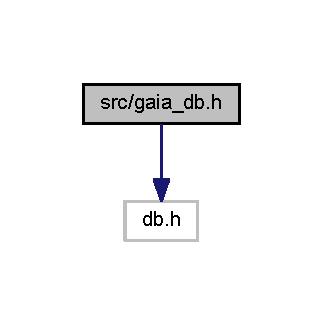
\includegraphics[width=155pt]{gaia__db_8h__incl}
\end{center}
\end{figure}
This graph shows which files directly or indirectly include this file\+:\nopagebreak
\begin{figure}[H]
\begin{center}
\leavevmode
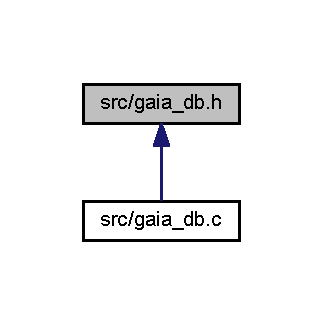
\includegraphics[width=155pt]{gaia__db_8h__dep__incl}
\end{center}
\end{figure}
\subsection*{Classes}
\begin{DoxyCompactItemize}
\item 
struct \mbox{\hyperlink{struct__star}{\+\_\+star}}
\begin{DoxyCompactList}\small\item\em Star struct which holds basic data of a star. \end{DoxyCompactList}\item 
struct \mbox{\hyperlink{struct__db__ctx}{\+\_\+db\+\_\+ctx}}
\begin{DoxyCompactList}\small\item\em A small struct which holds pointers to databases and the directory they are in. \end{DoxyCompactList}\end{DoxyCompactItemize}
\subsection*{Typedefs}
\begin{DoxyCompactItemize}
\item 
\mbox{\Hypertarget{gaia__db_8h_af49b70ce88035047e479faabf6e1593f}\label{gaia__db_8h_af49b70ce88035047e479faabf6e1593f}} 
typedef struct \mbox{\hyperlink{struct__star}{\+\_\+star}} \mbox{\hyperlink{gaia__db_8h_af49b70ce88035047e479faabf6e1593f}{S\+Star}}
\begin{DoxyCompactList}\small\item\em Star struct which holds basic data of a star. \end{DoxyCompactList}\item 
\mbox{\Hypertarget{gaia__db_8h_a35d505fe9a8343f69d3079cabcf0d402}\label{gaia__db_8h_a35d505fe9a8343f69d3079cabcf0d402}} 
typedef struct \mbox{\hyperlink{struct__db__ctx}{\+\_\+db\+\_\+ctx}} \mbox{\hyperlink{gaia__db_8h_a35d505fe9a8343f69d3079cabcf0d402}{D\+B\+\_\+\+C\+TX}}
\begin{DoxyCompactList}\small\item\em A small struct which holds pointers to databases and the directory they are in. \end{DoxyCompactList}\end{DoxyCompactItemize}
\subsection*{Functions}
\begin{DoxyCompactItemize}
\item 
\mbox{\hyperlink{gaia__db_8h_a35d505fe9a8343f69d3079cabcf0d402}{D\+B\+\_\+\+C\+TX}} $\ast$G\+A\+I\+A\+D\+B\+\_\+\+D\+LL \mbox{\hyperlink{gaia__db_8h_a43c8cb7ed007081547c637b25179131b}{gaia\+\_\+setup\+\_\+database}} (const char $\ast$directory)
\begin{DoxyCompactList}\small\item\em Setup the databases for G\+A\+IA. \end{DoxyCompactList}\item 
int G\+A\+I\+A\+D\+B\+\_\+\+D\+LL \mbox{\hyperlink{gaia__db_8h_a95196dc100fec9efbc68b8504ffe106f}{gaia\+\_\+close\+\_\+database}} (\mbox{\hyperlink{gaia__db_8h_a35d505fe9a8343f69d3079cabcf0d402}{D\+B\+\_\+\+C\+TX}} $\ast$context)
\begin{DoxyCompactList}\small\item\em Close the databases. Writes the db\textquotesingle{}s to a file. \end{DoxyCompactList}\item 
int G\+A\+I\+A\+D\+B\+\_\+\+D\+LL \mbox{\hyperlink{gaia__db_8h_ab0c2f8d166040d234e56d786b7a35eb1}{gaia\+\_\+new\+\_\+star}} (DB $\ast$dbp, u\+\_\+int64\+\_\+t id, double x, double y, double z, u\+\_\+int32\+\_\+t colour, float brightness, u\+\_\+int64\+\_\+t morton\+\_\+index)
\item 
\mbox{\hyperlink{gaia__db_8h_af49b70ce88035047e479faabf6e1593f}{S\+Star}} $\ast$G\+A\+I\+A\+D\+B\+\_\+\+D\+LL \mbox{\hyperlink{gaia__db_8h_adc9ab238094c0e19f4d7830a3c48e5ca}{gaia\+\_\+get\+\_\+star}} (DB $\ast$dbp, u\+\_\+int64\+\_\+t id)
\begin{DoxyCompactList}\small\item\em Get a star from the db based on the ID of the star. \end{DoxyCompactList}\item 
\mbox{\hyperlink{gaia__db_8h_af49b70ce88035047e479faabf6e1593f}{S\+Star}} $\ast$G\+A\+I\+A\+D\+B\+\_\+\+D\+LL \mbox{\hyperlink{gaia__db_8h_ae000cfd5cf46d177e00462153e4d3cb7}{gaia\+\_\+get\+\_\+star\+\_\+by\+\_\+morton}} (DB $\ast$sdbp, u\+\_\+int64\+\_\+t index)
\begin{DoxyCompactList}\small\item\em Get the star based on it\textquotesingle{}s morton code. \end{DoxyCompactList}\item 
int G\+A\+I\+A\+D\+B\+\_\+\+D\+LL \mbox{\hyperlink{gaia__db_8h_aa4475b8bfd3dfe389fdc0096f48af7ad}{gaia\+\_\+delete\+\_\+star}} (DB $\ast$dbp, u\+\_\+int64\+\_\+t id)
\begin{DoxyCompactList}\small\item\em Search and remove a star from the db. \end{DoxyCompactList}\item 
int G\+A\+I\+A\+D\+B\+\_\+\+D\+LL \mbox{\hyperlink{gaia__db_8h_aff8a02a9c2141ded3c9fea3e3ba17a70}{gaia\+\_\+update\+\_\+star\+\_\+morton}} (DB $\ast$dbp, u\+\_\+int64\+\_\+t id, u\+\_\+int64\+\_\+t morton\+\_\+index)
\begin{DoxyCompactList}\small\item\em Update the morton code of the star. \end{DoxyCompactList}\item 
D\+BC $\ast$G\+A\+I\+A\+D\+B\+\_\+\+D\+LL \mbox{\hyperlink{gaia__db_8h_abe434f04ea17b985dc6971ad55f00cfa}{gaia\+\_\+open\+\_\+cursor}} (DB $\ast$dbp)
\begin{DoxyCompactList}\small\item\em Get a new cursor to iterate over the database. \end{DoxyCompactList}\item 
char G\+A\+I\+A\+D\+B\+\_\+\+D\+LL \mbox{\hyperlink{gaia__db_8h_a06e8633beaa18999641c080f61ebb4cd}{gaia\+\_\+cursor\+\_\+has\+\_\+next}} (D\+BC $\ast$dbcp)
\begin{DoxyCompactList}\small\item\em Check if the cursor is on the last record and jump to that record. \end{DoxyCompactList}\item 
\mbox{\hyperlink{gaia__db_8h_af49b70ce88035047e479faabf6e1593f}{S\+Star}} $\ast$G\+A\+I\+A\+D\+B\+\_\+\+D\+LL \mbox{\hyperlink{gaia__db_8h_abce6dcda8b96c56f717254039107c09e}{gaia\+\_\+cursor\+\_\+get\+\_\+star}} (D\+BC $\ast$dbcp)
\begin{DoxyCompactList}\small\item\em Get the star the cursor is pointing to. \end{DoxyCompactList}\item 
int G\+A\+I\+A\+D\+B\+\_\+\+D\+LL \mbox{\hyperlink{gaia__db_8h_abe5eabfa1ec4a0af7349d554ace104ad}{gaia\+\_\+cursor\+\_\+goto\+\_\+star}} (D\+BC $\ast$dbcp, u\+\_\+int64\+\_\+t id)
\begin{DoxyCompactList}\small\item\em Set the cursor to a star with the id given. \end{DoxyCompactList}\item 
int G\+A\+I\+A\+D\+B\+\_\+\+D\+LL \mbox{\hyperlink{gaia__db_8h_a78ae970378513f914c0c627edcf457d4}{gaia\+\_\+close\+\_\+cursor}} (D\+BC $\ast$dbcp)
\begin{DoxyCompactList}\small\item\em Close the cursor after you are done using it. \end{DoxyCompactList}\end{DoxyCompactItemize}


\subsection{Detailed Description}
Gaia DB wrapper. 

\begin{DoxyAuthor}{Author}
Danny Dorstijn 
\end{DoxyAuthor}
\begin{DoxyVersion}{Version}
0.\+8 
\end{DoxyVersion}
\begin{DoxyDate}{Date}
2019-\/01-\/23
\end{DoxyDate}
\begin{DoxyCopyright}{Copyright}
Copyright (c) 2019 
\end{DoxyCopyright}


\subsection{Function Documentation}
\mbox{\Hypertarget{gaia__db_8h_a78ae970378513f914c0c627edcf457d4}\label{gaia__db_8h_a78ae970378513f914c0c627edcf457d4}} 
\index{gaia\+\_\+db.\+h@{gaia\+\_\+db.\+h}!gaia\+\_\+close\+\_\+cursor@{gaia\+\_\+close\+\_\+cursor}}
\index{gaia\+\_\+close\+\_\+cursor@{gaia\+\_\+close\+\_\+cursor}!gaia\+\_\+db.\+h@{gaia\+\_\+db.\+h}}
\subsubsection{\texorpdfstring{gaia\+\_\+close\+\_\+cursor()}{gaia\_close\_cursor()}}
{\footnotesize\ttfamily int G\+A\+I\+A\+D\+B\+\_\+\+D\+LL gaia\+\_\+close\+\_\+cursor (\begin{DoxyParamCaption}\item[{D\+BC $\ast$}]{dbcp }\end{DoxyParamCaption})}



Close the cursor after you are done using it. 


\begin{DoxyParams}{Parameters}
{\em dbcp} & -\/ Handle to the database \\
\hline
\end{DoxyParams}
\begin{DoxyReturn}{Returns}
int -\/ Error code or 0 if all is fine 
\end{DoxyReturn}
\mbox{\Hypertarget{gaia__db_8h_a95196dc100fec9efbc68b8504ffe106f}\label{gaia__db_8h_a95196dc100fec9efbc68b8504ffe106f}} 
\index{gaia\+\_\+db.\+h@{gaia\+\_\+db.\+h}!gaia\+\_\+close\+\_\+database@{gaia\+\_\+close\+\_\+database}}
\index{gaia\+\_\+close\+\_\+database@{gaia\+\_\+close\+\_\+database}!gaia\+\_\+db.\+h@{gaia\+\_\+db.\+h}}
\subsubsection{\texorpdfstring{gaia\+\_\+close\+\_\+database()}{gaia\_close\_database()}}
{\footnotesize\ttfamily int G\+A\+I\+A\+D\+B\+\_\+\+D\+LL gaia\+\_\+close\+\_\+database (\begin{DoxyParamCaption}\item[{\mbox{\hyperlink{gaia__db_8h_a35d505fe9a8343f69d3079cabcf0d402}{D\+B\+\_\+\+C\+TX}} $\ast$}]{ctx }\end{DoxyParamCaption})}



Close the databases. Writes the db\textquotesingle{}s to a file. 


\begin{DoxyParams}{Parameters}
{\em ctx} & -\/ The context with both the database handles \\
\hline
\end{DoxyParams}
\begin{DoxyReturn}{Returns}
int -\/ Returns err code or 0 if all was fine 
\end{DoxyReturn}
\mbox{\Hypertarget{gaia__db_8h_abce6dcda8b96c56f717254039107c09e}\label{gaia__db_8h_abce6dcda8b96c56f717254039107c09e}} 
\index{gaia\+\_\+db.\+h@{gaia\+\_\+db.\+h}!gaia\+\_\+cursor\+\_\+get\+\_\+star@{gaia\+\_\+cursor\+\_\+get\+\_\+star}}
\index{gaia\+\_\+cursor\+\_\+get\+\_\+star@{gaia\+\_\+cursor\+\_\+get\+\_\+star}!gaia\+\_\+db.\+h@{gaia\+\_\+db.\+h}}
\subsubsection{\texorpdfstring{gaia\+\_\+cursor\+\_\+get\+\_\+star()}{gaia\_cursor\_get\_star()}}
{\footnotesize\ttfamily \mbox{\hyperlink{gaia__db_8h_af49b70ce88035047e479faabf6e1593f}{S\+Star}}$\ast$ G\+A\+I\+A\+D\+B\+\_\+\+D\+LL gaia\+\_\+cursor\+\_\+get\+\_\+star (\begin{DoxyParamCaption}\item[{D\+BC $\ast$}]{dbcp }\end{DoxyParamCaption})}



Get the star the cursor is pointing to. 


\begin{DoxyParams}{Parameters}
{\em dbcp} & -\/ Handle to the database \\
\hline
\end{DoxyParams}
\begin{DoxyReturn}{Returns}
S\+Star$\ast$ -\/ The star the cursor is pointing to 
\end{DoxyReturn}
\mbox{\Hypertarget{gaia__db_8h_abe5eabfa1ec4a0af7349d554ace104ad}\label{gaia__db_8h_abe5eabfa1ec4a0af7349d554ace104ad}} 
\index{gaia\+\_\+db.\+h@{gaia\+\_\+db.\+h}!gaia\+\_\+cursor\+\_\+goto\+\_\+star@{gaia\+\_\+cursor\+\_\+goto\+\_\+star}}
\index{gaia\+\_\+cursor\+\_\+goto\+\_\+star@{gaia\+\_\+cursor\+\_\+goto\+\_\+star}!gaia\+\_\+db.\+h@{gaia\+\_\+db.\+h}}
\subsubsection{\texorpdfstring{gaia\+\_\+cursor\+\_\+goto\+\_\+star()}{gaia\_cursor\_goto\_star()}}
{\footnotesize\ttfamily int G\+A\+I\+A\+D\+B\+\_\+\+D\+LL gaia\+\_\+cursor\+\_\+goto\+\_\+star (\begin{DoxyParamCaption}\item[{D\+BC $\ast$}]{dbcp,  }\item[{u\+\_\+int64\+\_\+t}]{id }\end{DoxyParamCaption})}



Set the cursor to a star with the id given. 


\begin{DoxyParams}{Parameters}
{\em dbcp} & -\/ Handle to the database \\
\hline
{\em id} & -\/ ID to jump to \\
\hline
\end{DoxyParams}
\begin{DoxyReturn}{Returns}
int -\/ Error code or 0 if all is fine 
\end{DoxyReturn}
\mbox{\Hypertarget{gaia__db_8h_a06e8633beaa18999641c080f61ebb4cd}\label{gaia__db_8h_a06e8633beaa18999641c080f61ebb4cd}} 
\index{gaia\+\_\+db.\+h@{gaia\+\_\+db.\+h}!gaia\+\_\+cursor\+\_\+has\+\_\+next@{gaia\+\_\+cursor\+\_\+has\+\_\+next}}
\index{gaia\+\_\+cursor\+\_\+has\+\_\+next@{gaia\+\_\+cursor\+\_\+has\+\_\+next}!gaia\+\_\+db.\+h@{gaia\+\_\+db.\+h}}
\subsubsection{\texorpdfstring{gaia\+\_\+cursor\+\_\+has\+\_\+next()}{gaia\_cursor\_has\_next()}}
{\footnotesize\ttfamily char G\+A\+I\+A\+D\+B\+\_\+\+D\+LL gaia\+\_\+cursor\+\_\+has\+\_\+next (\begin{DoxyParamCaption}\item[{D\+BC $\ast$}]{dbcp }\end{DoxyParamCaption})}



Check if the cursor is on the last record and jump to that record. 


\begin{DoxyParams}{Parameters}
{\em dbcp} & -\/ Handle to the database \\
\hline
\end{DoxyParams}
\begin{DoxyReturn}{Returns}
char -\/ 1 if jump is succesful. Else 0 
\end{DoxyReturn}
\mbox{\Hypertarget{gaia__db_8h_aa4475b8bfd3dfe389fdc0096f48af7ad}\label{gaia__db_8h_aa4475b8bfd3dfe389fdc0096f48af7ad}} 
\index{gaia\+\_\+db.\+h@{gaia\+\_\+db.\+h}!gaia\+\_\+delete\+\_\+star@{gaia\+\_\+delete\+\_\+star}}
\index{gaia\+\_\+delete\+\_\+star@{gaia\+\_\+delete\+\_\+star}!gaia\+\_\+db.\+h@{gaia\+\_\+db.\+h}}
\subsubsection{\texorpdfstring{gaia\+\_\+delete\+\_\+star()}{gaia\_delete\_star()}}
{\footnotesize\ttfamily int G\+A\+I\+A\+D\+B\+\_\+\+D\+LL gaia\+\_\+delete\+\_\+star (\begin{DoxyParamCaption}\item[{DB $\ast$}]{dbp,  }\item[{u\+\_\+int64\+\_\+t}]{id }\end{DoxyParamCaption})}



Search and remove a star from the db. 


\begin{DoxyParams}{Parameters}
{\em dbp} & -\/ Handle for the primary database \\
\hline
{\em id} & -\/ The id of the star \\
\hline
\end{DoxyParams}
\begin{DoxyReturn}{Returns}
int -\/ Error code or 0 if all is fine 
\end{DoxyReturn}
\mbox{\Hypertarget{gaia__db_8h_adc9ab238094c0e19f4d7830a3c48e5ca}\label{gaia__db_8h_adc9ab238094c0e19f4d7830a3c48e5ca}} 
\index{gaia\+\_\+db.\+h@{gaia\+\_\+db.\+h}!gaia\+\_\+get\+\_\+star@{gaia\+\_\+get\+\_\+star}}
\index{gaia\+\_\+get\+\_\+star@{gaia\+\_\+get\+\_\+star}!gaia\+\_\+db.\+h@{gaia\+\_\+db.\+h}}
\subsubsection{\texorpdfstring{gaia\+\_\+get\+\_\+star()}{gaia\_get\_star()}}
{\footnotesize\ttfamily \mbox{\hyperlink{gaia__db_8h_af49b70ce88035047e479faabf6e1593f}{S\+Star}}$\ast$ G\+A\+I\+A\+D\+B\+\_\+\+D\+LL gaia\+\_\+get\+\_\+star (\begin{DoxyParamCaption}\item[{DB $\ast$}]{dbp,  }\item[{u\+\_\+int64\+\_\+t}]{id }\end{DoxyParamCaption})}



Get a star from the db based on the ID of the star. 


\begin{DoxyParams}{Parameters}
{\em dbp} & -\/ Handle for the primary database \\
\hline
{\em id} & -\/ ID of the star you are looking for \\
\hline
\end{DoxyParams}
\begin{DoxyReturn}{Returns}
S\+Star$\ast$ -\/ Star object with all the data corresponding to the id given 
\end{DoxyReturn}
\mbox{\Hypertarget{gaia__db_8h_ae000cfd5cf46d177e00462153e4d3cb7}\label{gaia__db_8h_ae000cfd5cf46d177e00462153e4d3cb7}} 
\index{gaia\+\_\+db.\+h@{gaia\+\_\+db.\+h}!gaia\+\_\+get\+\_\+star\+\_\+by\+\_\+morton@{gaia\+\_\+get\+\_\+star\+\_\+by\+\_\+morton}}
\index{gaia\+\_\+get\+\_\+star\+\_\+by\+\_\+morton@{gaia\+\_\+get\+\_\+star\+\_\+by\+\_\+morton}!gaia\+\_\+db.\+h@{gaia\+\_\+db.\+h}}
\subsubsection{\texorpdfstring{gaia\+\_\+get\+\_\+star\+\_\+by\+\_\+morton()}{gaia\_get\_star\_by\_morton()}}
{\footnotesize\ttfamily \mbox{\hyperlink{gaia__db_8h_af49b70ce88035047e479faabf6e1593f}{S\+Star}}$\ast$ G\+A\+I\+A\+D\+B\+\_\+\+D\+LL gaia\+\_\+get\+\_\+star\+\_\+by\+\_\+morton (\begin{DoxyParamCaption}\item[{DB $\ast$}]{sdbp,  }\item[{u\+\_\+int64\+\_\+t}]{index }\end{DoxyParamCaption})}



Get the star based on it\textquotesingle{}s morton code. 


\begin{DoxyParams}{Parameters}
{\em sdbp} & -\/ Handle for the secondary database with morton code indices \\
\hline
{\em index} & -\/ The morton code index \\
\hline
\end{DoxyParams}
\begin{DoxyReturn}{Returns}
S\+Star$\ast$ -\/ The star data corresponding to the index given 
\end{DoxyReturn}
\mbox{\Hypertarget{gaia__db_8h_ab0c2f8d166040d234e56d786b7a35eb1}\label{gaia__db_8h_ab0c2f8d166040d234e56d786b7a35eb1}} 
\index{gaia\+\_\+db.\+h@{gaia\+\_\+db.\+h}!gaia\+\_\+new\+\_\+star@{gaia\+\_\+new\+\_\+star}}
\index{gaia\+\_\+new\+\_\+star@{gaia\+\_\+new\+\_\+star}!gaia\+\_\+db.\+h@{gaia\+\_\+db.\+h}}
\subsubsection{\texorpdfstring{gaia\+\_\+new\+\_\+star()}{gaia\_new\_star()}}
{\footnotesize\ttfamily int G\+A\+I\+A\+D\+B\+\_\+\+D\+LL gaia\+\_\+new\+\_\+star (\begin{DoxyParamCaption}\item[{DB $\ast$}]{dbp,  }\item[{u\+\_\+int64\+\_\+t}]{id,  }\item[{double}]{x,  }\item[{double}]{y,  }\item[{double}]{z,  }\item[{u\+\_\+int32\+\_\+t}]{colour,  }\item[{float}]{brightness,  }\item[{u\+\_\+int64\+\_\+t}]{morton\+\_\+index }\end{DoxyParamCaption})}


\begin{DoxyParams}{Parameters}
{\em dbp} & -\/ Handle for the primary db \\
\hline
{\em id} & -\/ ID of the star extracted from the uuid in the gaia dataset \\
\hline
{\em x} & -\/ X position of the star \\
\hline
{\em y} & -\/ Y position of the star \\
\hline
{\em z} & -\/ Z position of the star \\
\hline
{\em colour} & -\/ The colour of the star \\
\hline
{\em brightness} & -\/ The brightness of the star (apparent magnitude) \\
\hline
{\em morton\+\_\+index} & -\/ The morton index of the star. Leave 0 if unsure \\
\hline
\end{DoxyParams}
\begin{DoxyReturn}{Returns}
int -\/ Error code or 0 if fine 
\end{DoxyReturn}
\mbox{\Hypertarget{gaia__db_8h_abe434f04ea17b985dc6971ad55f00cfa}\label{gaia__db_8h_abe434f04ea17b985dc6971ad55f00cfa}} 
\index{gaia\+\_\+db.\+h@{gaia\+\_\+db.\+h}!gaia\+\_\+open\+\_\+cursor@{gaia\+\_\+open\+\_\+cursor}}
\index{gaia\+\_\+open\+\_\+cursor@{gaia\+\_\+open\+\_\+cursor}!gaia\+\_\+db.\+h@{gaia\+\_\+db.\+h}}
\subsubsection{\texorpdfstring{gaia\+\_\+open\+\_\+cursor()}{gaia\_open\_cursor()}}
{\footnotesize\ttfamily D\+BC$\ast$ G\+A\+I\+A\+D\+B\+\_\+\+D\+LL gaia\+\_\+open\+\_\+cursor (\begin{DoxyParamCaption}\item[{DB $\ast$}]{dbp }\end{DoxyParamCaption})}



Get a new cursor to iterate over the database. 


\begin{DoxyParams}{Parameters}
{\em dbp} & -\/ Handle to the database \\
\hline
\end{DoxyParams}
\begin{DoxyReturn}{Returns}
D\+B\+C$\ast$ -\/ The cursor 
\end{DoxyReturn}
\mbox{\Hypertarget{gaia__db_8h_a43c8cb7ed007081547c637b25179131b}\label{gaia__db_8h_a43c8cb7ed007081547c637b25179131b}} 
\index{gaia\+\_\+db.\+h@{gaia\+\_\+db.\+h}!gaia\+\_\+setup\+\_\+database@{gaia\+\_\+setup\+\_\+database}}
\index{gaia\+\_\+setup\+\_\+database@{gaia\+\_\+setup\+\_\+database}!gaia\+\_\+db.\+h@{gaia\+\_\+db.\+h}}
\subsubsection{\texorpdfstring{gaia\+\_\+setup\+\_\+database()}{gaia\_setup\_database()}}
{\footnotesize\ttfamily \mbox{\hyperlink{gaia__db_8h_a35d505fe9a8343f69d3079cabcf0d402}{D\+B\+\_\+\+C\+TX}}$\ast$ G\+A\+I\+A\+D\+B\+\_\+\+D\+LL gaia\+\_\+setup\+\_\+database (\begin{DoxyParamCaption}\item[{const char $\ast$}]{directory }\end{DoxyParamCaption})}



Setup the databases for G\+A\+IA. 


\begin{DoxyParams}{Parameters}
{\em directory} & -\/ The base directory to put the databases in \\
\hline
\end{DoxyParams}
\begin{DoxyReturn}{Returns}
D\+B\+\_\+\+C\+T\+X$\ast$ -\/ A helper to manage the databases 
\end{DoxyReturn}
\mbox{\Hypertarget{gaia__db_8h_aff8a02a9c2141ded3c9fea3e3ba17a70}\label{gaia__db_8h_aff8a02a9c2141ded3c9fea3e3ba17a70}} 
\index{gaia\+\_\+db.\+h@{gaia\+\_\+db.\+h}!gaia\+\_\+update\+\_\+star\+\_\+morton@{gaia\+\_\+update\+\_\+star\+\_\+morton}}
\index{gaia\+\_\+update\+\_\+star\+\_\+morton@{gaia\+\_\+update\+\_\+star\+\_\+morton}!gaia\+\_\+db.\+h@{gaia\+\_\+db.\+h}}
\subsubsection{\texorpdfstring{gaia\+\_\+update\+\_\+star\+\_\+morton()}{gaia\_update\_star\_morton()}}
{\footnotesize\ttfamily int G\+A\+I\+A\+D\+B\+\_\+\+D\+LL gaia\+\_\+update\+\_\+star\+\_\+morton (\begin{DoxyParamCaption}\item[{DB $\ast$}]{dbp,  }\item[{u\+\_\+int64\+\_\+t}]{id,  }\item[{u\+\_\+int64\+\_\+t}]{morton\+\_\+index }\end{DoxyParamCaption})}



Update the morton code of the star. 


\begin{DoxyParams}{Parameters}
{\em dbp} & -\/ Handle of the primary database \\
\hline
{\em id} & -\/ The id of the star \\
\hline
{\em morton\+\_\+index} & -\/ The new morton index \\
\hline
\end{DoxyParams}
\begin{DoxyReturn}{Returns}
int -\/ Error code or 0 if all is fine 
\end{DoxyReturn}

%--- End generated contents ---

% Index
\backmatter
\newpage
\phantomsection
\clearemptydoublepage
\addcontentsline{toc}{chapter}{Index}
\printindex

\end{document}
